\chapter{Comparison}%
	\label{ch:comparison}%
  \index{Estimation (statistical)}%
	\index{Significance (statistical)}

This chapter deals with two classes of quantitative comparisons:

\begin{itemize}
  \item \emph{Confidence intervals} are a form of comparison of the distribution of a variable against the same amount of normally distributed data. %
  \item \emph{Significance tests} are a form of comparison of a variation in the data against the same extent of variation in a random sample. %
\end{itemize}

These topics are given different names in statistical theory:

\begin{itemize}
  \item \emph{Estimation} is the generic way to designate methods that allow to generalize the parameters of a sample to a target population. This is what you want to do when you have a sample of American adults and want to estimate in what bounds the average weight of the entire American adult population is likely to lie. The same principle applies when you are estimating a proportion, such as the likely proportion of adults who will vote for a given political candidate in the next election. %
  \item \emph{Hypothesis testing} is the generic way to address the test of a parameter against the ``null hypothesis''.
\end{itemize}

\newthought{A hypothesis} is a statement that you can either confirm or contradict. ``People at the extremes are happier than political moderates \dots none, it seems, are happier than the Tea Partiers \dots'', for instance, is a verifiable statement that happens to be false in the context in which it was formulated.\footnote{The statement is from a \emph{New York Times} article by Arthur Brooks. See Jay Livingston's blog, ``\href{http://montclairsoci.blogspot.ch/2012/07/bitter-tea.html}{Bitter Tea?}'' (10 July 2012), and Andrew Gelman's blog, ``\href{http://andrewgelman.com/2012/08/1-5-million-people-were-told-that-extreme-conservatives-are-happier-than-political-moderates-approximately-0001-million-americans-learned-that-the-opposite-is-true/}{1.5 million people were told that extreme conservatives are happier than political moderates. Approximately .0001 million Americans learned that the opposite is true}'' (14 August 2012).} You can verify this yourself by looking into the U.S. General Social Survey from 2010:%

\begin{verbatim}
use datasets/gss2010, clear
spineplot happy partyid if partyid < 7 [aw=wtssall], ///
    xla(, alt axis(2)) xti("", axis(2)) scheme(set1)
\end{verbatim}

The \cmd{spineplot} command above displays proportions of the sample by level of subjective happiness (\texttt{happy}) and political party affiliation (\texttt{partyid}, with over 97\% of the respondents placing themselves on a scale ranging from 0 ``Strong Democrat'' to 6 ``Strong Republican''). The graph options on the last line are optional.

The result visually contradicts the previous statement by suggesting a more ambiguous relationship between the two variables:

\begin{figure}
  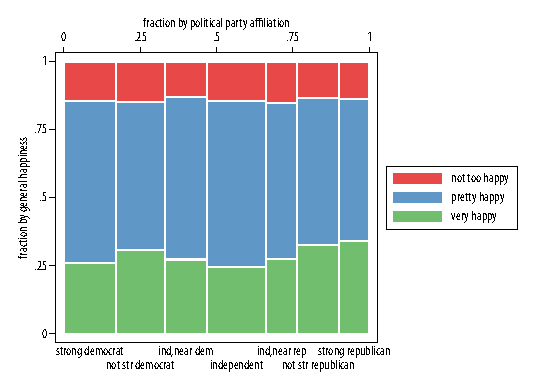
\includegraphics{gss-happy}
  \caption[Subjective happiness by political affiliation.]%
  {Subjective happiness by political affiliation. %
  \emph{The General Social Survey, which started in 1972, has repeatedly measured both variables over the years. The pattern suggested by Arthur Brooks holds when the data are averaged over the years, but it visibly does not hold for 2010.}}%
  \label{fig:stata-window}
\end{figure}

\newthought{Hypothesis testing} is a way to test your data against a hypothesis. Statistical significance tests do so by assuming that you want to compare your data against randomness, in order to prove that the associations you observe in the data are very unlikely to be due to an accidental sampling error. The `hypothesis' in `hypothesis testing' is therefore the possibility of an association in the data being random. This is denoted $H_0$ and called the \emph{null hypothesis}.

More generally, the null hypothesis assesses something like this:

\begin{quote}
If the data were generated randomly, how likely is it that we would obtain a pattern identical to the one that we observe in the sample?
\end{quote}

\newthought{Rejecting the null hypothesis} involves specifying what the null hypothesis might be. If you are inspecting income by gender, it might be that the average income is lower among females than among males. If you are exploring party affiliation and subjective well-being, it might simply be the existence of an association between the two variables. 

Intuitively, your \emph{substantive} hypothesis is that an association or a difference \emph{does} exist in the data. Statistics do not take over your hypothesis, and instead offer you the possibility to prove it by contradiction, by rejecting the null hypothesis of an accidental association that could also exist in randomly generated data.

\newthought{Statistical significance} characterizes an association for which the null hypothesis is highly unlikely. The common 95\% and 99\% levels of confidence are conventional thresholds at which you can choose to reject the null hypothesis. At these thresholds, the probability of the null hypothesis is respectively $p < .05$ and $p < .01$.\footnote{The probability of the null hypothesis $H_0$ is called the $p$-value and the level of statistical significance at which you reject $H_0$ is called $\alpha$.}

\newthought{Be careful:} the probability of your substantive hypothesis, denoted $H_a$ for ``alternative hypothesis'', is \emph{not} equal to $1 - p$. The low probability that there is no association \emph{at all} in the data does not mean that your specific hypothesis on that association is correct.

Take, for instance, this abstract from a U.S. libertarian think tank (emphasis added):

\begin{quote}
A number of theorists assume that drinking has harmful economic effects, but data show that drinking and earnings are positively correlated. \textbf{We hypothesize that drinking leads to higher earnings by increasing social capital.} If drinkers have larger social networks, their earnings should increase. Examining the General Social Survey, we find that self-reported drinkers earn 10-14 percent more than abstainers, which replicates results from other data sets. We then attempt to differentiate between social and nonsocial drinking by comparing the earnings of those who frequent bars at least once per month and those who do not. We find that males who frequent bars at least once per month earn an additional 7 percent on top of the 10 percent drinkers' premium. These results suggest that social drinking leads to increased social capital.\footnote{The abstract is from a Reason Foundation report by Bethany L. Peters and Edward Stringham, ``\href{http://reason.org/news/show/127594.html}{No Booze? You May Lose. Why Drinkers Earn More Money Than Nondrinkers}'' (September 2006).}
\end{quote}

In this study, if the null hypothesis $H_0$ is the absence of any association between earnings and drinking, then the presence of a relationship is hardly surprising. However, the probability of that relationship is \emph{not} equal to the probability of the alternative hypothesis $H_a$ stating that ``drinking leads to higher earnings'', as the reverse statement might also be true to some (possibly wider) extent.\footnote{Devise at least two reasons why the causality might run from high income to frequent social drinking, rather than vice versa. I owe this question and example to \href{https://pinboard.in/u:cshalizi/b:d54b8c984beb}{Cosma Shalizi}.}

\newthought{Furthermore,} rejecting the null hypothesis while it is actually true, or the reverse error, is still a possible outcome of your interpretation of the test. 

\newthought{Statistical significance has no effect on bias.} If your sample, measurements or hypotheses are biased, or if your reporting of their tests is, then you are left with an entirely different set of issues to deal with. The problem is ubiquitous among all branches of contemporary science:

\begin{quote}
There is increasing concern that most current published research findings are false. The probability that a research claim is true may depend on study power and bias, the number of other studies on the same question, and, importantly, the ratio of true to no relationships among the relationships probed in each scientific field. In this framework, a research finding is less likely to be true when the studies conducted in a field are smaller; when effect sizes are smaller; when there is a greater number and lesser preselection of tested relationships; where there is greater flexibility in designs, definitions, outcomes, and analytical modes; when there is greater financial and other interest and prejudice; and when more teams are involved in a scientific field in chase of statistical significance\cite{Ioannidis:2005u}.
\end{quote}

To minimize bias, first make sure that you fully understand the limitations of your dataset and variables. Then, make sure that you formulate your hypotheses in the clearest possible way. Finally, report both negative and positive findings for which you have both a statistical significance test and some observation to substantiate its result.


%
%
%
\section{Confidence intervals}

	%
	% 4.1.1
	%
	\subsection{Applying the ``CLT''}

	%
	% 4.1.2
	%
	\subsection{Estimating a ``95\% CI''}
%
%
%
%
%
\section{Significance tests}

	%
	% 4.2.1
	%
	\subsection{Comparing two means}

	%
	% 4.2.2
	%
	\subsection{Comparing two proportions}
%
%
%
%
%
\section{Crosstabulations}

	%
	% 4.3.1
	%
	\subsection{Chi-squared test}

	%
	% 4.3.2
	%
	\subsection{Odds ratios}
%
%
